%%\documentclass[preprint,10pt]{sigplanconf}
%%\documentclass[10pt]{journal}
%%\documentclass[preprint, 10pt]{sigplanconf}



\documentclass{acm_proc_article-sp-sigmod09}

%%\usepackage{amsthm}


\usepackage[usenames, dvipsnames]{color}
\usepackage{times}
%%\usepackage{url}
%%\usepackage{graphicx}
%%\usepackage{boxedminipage}
\usepackage{xspace}
\usepackage{textcomp}
\usepackage{wrapfig}
\usepackage{url}
%%\usepackage{verbatim}
%%\usepackage{latexsym}
\usepackage{amsmath, amssymb}
%%\usepackage{amsthm}

\usepackage{alltt}
\usepackage{appendix}


\newcommand{\jmh}[1]{{\textcolor{red}{#1 -- jmh}}}
\newcommand{\paa}[1]{{\textcolor{blue}{#1 -- paa}}}
\newcommand{\rcs}[1]{{\textcolor{green}{#1 -- rcs}}}
\newcommand{\nrc}[1]{{\textcolor{magenta}{#1 -- nrc}}}
\newcommand{\wrm}[1]{{\color{BurntOrange}{#1 -- wrm}}}
\newcommand{\smallurl}[1]{{\small \url{#1}}}

%dedalus environment for code
\newenvironment{Dedalus}{
\vspace{0.5em}\begin{minipage}{0.95\textwidth}%\linespread{1.3}
\begin{alltt}\fontsize{9pt}{9pt}\selectfont}
{\end{alltt}\end{minipage}\vspace{0.5em}}

\newcommand{\dedalus}[1]{\texttt{\fontsize{9pt}{9pt}\selectfont #1}}

\begin{document}
%
% --- Author Metadata here ---
\conferenceinfo{ACM PODS}{'10 Indianapolis, IN, USA}
%\setpagenumber{50}
%\CopyrightYear{2002} % Allows default copyright year (2002) to be over-ridden - IF NEED BE.
%\crdata{0-12345-67-8/90/01}  % Allows default copyright data (X-XXXXX-XX-X/XX/XX) to be over-ridden.
% --- End of Author Metadata ---

\title{Dedalus\titlenote{\small
Dedalus is intended as a precursor language for \textbf{Bloom}, a high-level language for programming distributed systems that
will replace Overlog in the \textbf{BOOM} project~\cite{boom-techr}.  
As such, it is derived from the character Stephen Dedalus in James Joyce's \emph{Ulysses}, whose dense and precise chapters 
precede those of the novel's hero, Leopold Bloom.  The character Dedalus, in turn, was partly derived from Daedalus, the greatest
of the Greek engineers and father of Icarus.  Unlike Overlog, which flew too close to the sun, Dedalus remains firmly grounded.
}: 
Datalog in Space and Time} 
%%Format\titlenote{(Produces the permission block, copyright information and page numbering). For use with ACM\_PROC\_ARTICLE-SP.CLS V2.6SP. Supported by ACM.}}
%
% You need the command \numberofauthors to handle the "boxing"
% and alignment of the authors under the title, and to add
% a section for authors number 4 through n.

\numberofauthors{5}

\author{Peter Alvaro, Neil Conway, William R. Marczak, Joseph M. Hellerstein, David Maier}
%%\author{Neil Conway}

\maketitle

\begin{abstract}

why does anyone care?

\begin{itemize}
\item Dedalus is not a new formalism, but an application of an existing formalism (under certain constraints) to new application domains.
\item Dedalus moves many tricky issues for updatable and distributed deductive databases (including table persistence, update, key constraints, and message delay and loss) from ambiguous type systems and operational semantics into the language itself, giving a logical interpretation for each.
\item Moreover, dedalus exposes the minimum necessary language constructs to capture those temporal details that affect program semantics.  This has
implications both for implementing and locally modeling distributed systems.
\end{itemize}
\end{abstract}

\section{Introduction} 
\label{sec:intro} 
Although distributed programming has become an essential and commonplace task,
it remains very challenging for most developers to write correct distributed
programs. The inherent difficulties of distributed computing---concurrency,
asynchrony, and partial failure---are exacerbated by the scale at which modern
distributed systems operate.

% remind reviewers that it's a database problem. can remove if accepted! 
Much of the discussion about distributed programming today revolves around data
management systems, and the tradeoffs between transactions and loose
consistency. Programmers using distributed transactions are relieved of
consistency concerns but often face significant performance and operational
challenges~\cite{Birman2009}. By contrast, programmers who use loosely
consistent systems can expect more predictable and low-latency performance, but
must reason explicitly about program correctness over inconsistent distributed
state.

In recent years there has been increased interest in techniques to help
programmers achieve correct program behavior without requiring strongly
consistent storage. This idea has been explored in two different frameworks,
\emph{Convergent Objects} and \emph{Monotonic Logic}.

\vspace{0.5em}\noindent
\textbf{Convergent Objects}: In this approach, a programmer writes encapsulated
object classes whose public methods guarantee certain properties regarding
message reordering and/or retry. For example, Statebox is an open-source library
that merges conflicting updates to data items in a key-value store; the user of
the library need only register commutative, idempotent merge
functions~\cite{statebox}. This approach has roots in research in
databases~\cite{Farrag1989,Garcia-Molina1983,Helland2009} and
groupware~\cite{Ellis1989,Sun1998}.  Shapiro et al.\ recently proposed a model
for these approaches called \emph{Conflict-Free Replicated Data Types} (CRDTs),
which formalizes these ideas in an algebraic framework~\cite{Shapiro2011b}.

The main problem with the CRDT approach is that its guarantees of correctness
are limited to an individual replicated data value, not to application logic in
general. For example, consider a distributed algorithmic trading service that
uses a CRDT to represent a mutable set \texttt{Portfolio}. Suppose one server
$M$ reads a local version of the set containing an element \texttt{BNNA} and
constructs an expected portfolio value $v = f(\mbox{\texttt{Portfolio}})$
derived from that version. Concurrently, \texttt{BNNA} is removed from the local
version of \texttt{Portfolio} at another server $N$. The CRDT can ensure that
$M$ and $N$ will eventually agree that \texttt{BNNA} is absent from the set, but
the application state at $M$ and $N$ may remain inconsistent unless the value
$v$ at $M$ is updated to reflect the removal of \texttt{BNNA}. Although the CRDT
maintains its own invariants, the programmer still bears the burden of ensuring
the consistency semantics of the entire program.

\vspace{0.5em} \noindent
\textbf{Monotonic Logic}: In recent work, we observed that the database theory
literature on non-monotonic logic provides a promising starting point for
reasoning about distributed consistency. Intuitively, a \emph{monotonic} program
computes more information over time---it never ``retracts'' an earlier
conclusion in the face of new information. We proposed the CALM
theorem~\cite{Hellerstein2010}, which established that all monotonic programs
are eventually consistent~\cite{Ameloot2011,dedalus-pods12-tr}. Monotonicity of
a Datalog-style program is straightforward to determine conservatively from
syntax, so the CALM theorem provides the basis for a simple analysis technique
for verifying the consistency of distributed programs~\cite{Alvaro2011}. We
realized the CALM analysis as part of Bloom, a Datalog-based DSL for distributed
programming~\cite{bloom}.

The original formulation of Bloom and CALM only validated consistency for programs that compute sets of facts that grow over time (``set monotonicity''); that is, ``growth'' is defined according to set containment. As a practical matter, this is overly conservative: several common distributed programming idioms that are monotonic do not satisfy syntactic monotonicity tests for Datalog. In particular, threshold tests over monotonic aggregate values (e.g., ``$\mathrm{max}(S) > k$'') and upward-moving mutable counters are both considered to be non-monotonic by the original CALM analysis.  As a result, the initial Bloom prototype advises the programmer to guard those constructs with strong consistency methods like Paxos~\cite{Lamport1998} or Two-Phase Commit. 

\subsection{A Hybrid Approach}
% The strengths and weaknesses of these two approaches appear complementary. CRDTs provide synchronization-free consistent objects, but cannot guarantee whole-program consistency. Bloom's CALM analysis guarantees whole-program consistency but is unable to verify a number of natural coordination-free mechanisms.
In this paper, we extend our previous work to accommodate the ideas underlying CRDTs. Instead of only allowing growth according to the set containment
partial order, we allow any user-defined partial order to be used.  
We do this by providing \emph{join semi-lattices} as a programming construct.
We give a
formal definition of this construct below, but the intuition is that the programmer provides a commutative, idempotent merge function (``least upper bound'')
that takes two input values and produces an output value that is not smaller
than either of the input values (according to the user's partial order). This
generalizes Bloom (and traditional Datalog), which assumes a fixed merge
function (set union) and partial order (set containment).
% Relate user-defined merge functions to merge functions in other contexts?
% (e.g., key-value store, COPS, Piccolo)

% Explain how lattices generalize monotonic datalog
It is attractive to incorporate join semi-lattices into logic programming,  but doing so raises challenges in language design, consistency analysis and efficient execution.  In this paper, we make the following contributions:
\begin{enumerate}
% \item
%   We present \baselang, a variant of Datalog that is defined over lattices. We
%   define a model-theoretic semantics for \baselang, and show that \baselang
%   generalizes Datalog.

\item
  We introduce \lang, an extension of Bloom that supports lattices. We detail
  the builtin lattice types provided by \lang and show how developers can
  define new lattices.
  
\item 
  We provide interfaces for consistency-preserving mappings across lattices via
  \emph{morphisms} and \emph{monotonic functions}.  This is critical for \lang
  and forms a useful extension to the CRDT framework as well.

\item 
  We generalize the CALM analysis to programs that contain both lattices and
  set-oriented collections, and show how lattices can be used to prove the
  confluence of several common distributed design patterns that were regarded as
  non-monotonic in Bloom. % XXX: revisit this

\item
  For efficient execution, we show how to extend the standard Datalog semi-naive
  evaluation scheme~\cite{Balbin1987} to support both lattices and traditional
  database relations. We also describe how an existing Datalog engine can be
  extended to support lattices with relatively minor changes.

\item
  Finally, we demonstrate the usefulness of lattices with two case studies.
  First we revisit the simple e-commerce scenario presented in Alvaro et al., in
  which clients interact with a replicated shopping cart
  service~\cite{Alvaro2011}. We show how \lang can be used to make the
  ``checkout'' operation monotonic, despite the fact that it requires
  aggregating over a distributed data set.

  Second, we use \lang to implement vector clocks and causal delivery, two
  standard building blocks for distributed programming. We show how both
  algorithms can be realized as monotonic \lang programs that are concise and
  readable.
\end{enumerate}

\section{Related Work}
\label{sec:relwork}
The shopping cart case study in Section~\ref{sec:case} was motivated by the
Amazon Dynamo paper~\cite{dynamo}, as well as the related discussion by Helland
and Campbell~\cite{quicksand}. Systems with loose consistency requirements have
been explored in depth by both the systems and database management communities
(e.g.,~\cite{sagas,leases,dangers,bayou}); we do not attempt to provide
an exhaustive survey here.

The Bloom language is inspired by earlier work that attempts to integrate
databases and programming languages.  This includes early research such as
Gem~\cite{gem} and more recent object-relational mapping layers like Ruby on
Rails.  Unlike these efforts, Bloom is targeted at the development of both
distributed infrastructure and distributed applications, so it does not make any
assumptions about the presence of a database system ``underneath it.''  Given
our prototype implementation in Ruby, it is tempting to integrate Bud with
Rails; we have left this for future work.

Our work on Bloom bears a resemblance to the Reactor
language~\cite{reactors}. Both languages target distributed programming and are
grounded in Datalog. Moreover, both languages combine declarative rules and
state into a single program construct. While Bloom uses a syntax inspired by
object-oriented languages, Reactor takes a more explicitly agent-oriented
approach. Reactor also includes synchronous coupling between agents as a
primitive; we have opted to only include asynchronous communication as a
language primitive and to provide synchronous coordination between nodes as a
library. Another significant different is that, like many rule-based languages,
Reactor includes some imperative constructs (e.g., \ldots), whereas rules in
Bloom are purely declarative.

Another recent language related to our work is Coherence~\cite{coherence}, which
also embraces ``disorderly'' programming. Unlike Bloom, Coherence is not
designed for distributed computing and is not based on logic programming.

There is a long history of attempts to design programming languages more
suitable to parallel and distributed systems; for example, Argus~\cite{argus}
and Linda~\cite{linda}.  Again, we do not hope to survey that literature here.
More pragmatically, Erlang is an oft-cited choice for distributed programming in
recent years.  Erlang's features and design style encourage the use of
asynchronous lightweight ``actors.''  As mentioned previously, we did a simple
Bloom prototype DSL in Erlang (which we cannot help but call ``Bloomerlang''),
and there is a natural correspondence between Bloom-style distributed rules and
Erlang actors.  However there is no requirement for Erlang programs to be
written in the disorderly style of Bloom. It is not obvious that typical Erlang
programs are significantly more amenable to a useful points-of-order analysis
than programs written in any other functional language.  For example, ordered
lists are basic constructs in functional languages, and without program
annotation or deeper analysis than we need to do in Bloom, any code that
modifies lists would need be marked as a point of order, much like our
destructive shopping cart.  We believe that Bloom's ``disorderly by default''
style encourages more disorderly programming; we know that its roots in database
theory bore fruit in terms of our analysis.  While we would be happy to see the
analysis ``ported'' to currently popular distributed programming environments,
it may be that design patterns using Bloom-esque disorderly programming are the
natural way to achieve this.

\section{Dedalus}

By reifying time as data, we are able to reason about time in our logic.  some useful things fall out of this right away: persistence is now programatic rather than a separate type, ditto key constraints.  event creation vs. effect ambiguities are resolved.

Perhaps more importantly, the infinite sequence of abstract time gives us a way to reason about ordering, which is particularly difficult in a set-oriented language like Datalog.  The ordering over any program inputs (e.g. message queues) can be represented as a mapping between the ordering domain of the input and the time relation.

\subsection{Syntax}

A Dedalus program is a Datalog program in which every predicate is annotated with a time suffix.  A Dedalus predicate has the following form:

$p(A_{1}, A_{2}, [...], A_{n})@S$

The predicate p() is a truth-valued function over its arguments $A_{1} - A_{n}$, which may be of any type, and S, which is an integer expression 
referring to the logical clock time at which the predicate holds, taking one of the following three suffix forms:

\begin{enumerate}
\item $N$
\item $N + 1$
\item $N + r(A_{1}, A_{2}, [...], A_{n})$
\item an integer
\end{enumerate}

Facts and rules in Dedalus are 
defined just as in Datalog, with the additional restrictions:

\begin{itemize}
\item Every body predicate may only have the suffix $N$.
\item A head predicate may have any suffix except a constant integer.
\item A fact must be posited with a constant integer for S, or the special function now().
\end{itemize}
Rules with the head suffix $N$ are called \emph{deductive} or atemporal rules, and describe all the logical consequences of facts in a given 
timestep. Deductive rules may be interpreted as pure Datalog rules by dropping the suffixes, treating all facts that are true in the current 
timestep as Datalog EDB, and running the rules to fixpoint.

Rules with the head suffix $N + 1$ are called \emph{inductive} temporal rules, and describe the relationship between facts in the current timestep 
and their consequences in the immediate next timestep. Inductive rules allow us to atomically capture change in time, and to model persistent state.

Rules with the head suffix $N+r(_)$ are also temporal rules, but unlike inductive rules, they carry no guarantee as to in which timestep, if any, 
their consequences will become visible. Such rules, called message rules, allow us to model network messages between nodes: the nodes 
are likely to have different clock values, and messages may be lost or delayed arbitrarily.

\subsubsection{Events}

An event in Dedalus corresponds to a Datalog fact.  It is a bodyless head clause with all constant terms in the form


$p(C_{1},C_{2},[...],C_{n})@I;$


where the elements of C are constants of any type and I is an integer constant.

Events provide ground for any logical inferences given by the deductive rules of the program, and may provide ground for inferences at 
future time steps via inductive rules.

\subsubsection{Persistence}

Events are only true at a single timestep.  It might seem that we could express a persistent predicate as a Datalog fact with a free variable 
for the time suffix.  The tuple would then be universally quantified over time:

\begin{Dedalus}
p(a, b)@N;
\end{Dedalus}

But clearly, because this must be interpreted as a rule head with an unbound variable, it produces an unsafe rule.  Instead, persistence is
expressed by an inductive rule that projects a tuple into the next timestep:

\begin{Dedalus}
p(a, b)@N+1 \(\leftarrow\)
  p(a, b)@N, 
  \(\lnot\) del\_p(a, b)@N;
\end{Dedalus}

This rule, in turn, may be viewed as informally equivalent to a rule in which the inductive step is driven by an 
explicit successor relation, and in which the time suffixes are attributes of their respective predicates:

\begin{Dedalus}
p(a, b, S) \(\leftarrow\)
  p(a, b, N),
  successor(N, S), 
  \(\lnot\) del\_p(a, b, N);
\end{Dedalus}

The final subgoal /emph{del\_p} allows us to model overwriteable storage: without it, a tuple will be trivially true at every future timestep if it becomes true
at any timestep.  Consider the following trace of events:

\begin{Dedalus}
p(1,2)@101;
p(1,3)@102;
p(1,?)@200;
del_p(1,2)@300;
p(1,?)@301;
\end{Dedalus}

It is easy to see that the results of the two queries are:


\begin{Dedalus}
p(1,2)@200;
p(1,3)@200;
p(1,3)@301;
\end{Dedalus}

\subsubsection{State Change}

Under this interpretation, a database update is an atomic (due to the adjacent timestamps)
pair of events with a deletion of the old value and assertion of the new, in the form:

$p(C_{1},C_{2},[...],C_{n})@I;$
\\
$del\_p(C_{1},C_{2},[...],C_{n})@I+1;$

For example:

\begin{Dedalus}
del\_p(1,2)@300; 
p(1, 4)@301;
\end{Dedalus}

\subsubsection{Sequences}

\begin{Dedalus}
seq(Agent, S + 1)@N+1 \(\leftarrow\)
  seq(Agent, S)@N, 
  event(Agent)@N; 
  
seq(Agent, S)@N+1 \(\leftarrow\) 
  seq(Agent, S)@N, 
  \(\lnot\) event(Agent)@N;
\end{Dedalus}

\subsection{Semantics}


\subsubsection{Static Interpretation}
\newtheorem{theorem}{Theorem}

\begin{theorem}
Every Dedalus program P with only deductive rules is equivalent to a Datalog program P'.
\end{theorem}

\begin{proof}
All rules in such a program will be in the form (shown propositionally for simplicity): 

%%\begin{Dedalus}
$p@N \leftarrow b_{1}@N, b_{2}@N, [...], b_{n}@N$
%%\end{Dedalus}

Where p is a head predicate and the $b$s are body predicates.  Note that all time suffixes are 
the same.

Because the time suffix is outside the scope of Datalog, a Datalog fact in the form:

$q(A_{1}, A_{2}, [...], A_{n});$

may be interpreted (equivalently) as persistently true (hence quantified over all logical times $N$) or instantaneously
true at some N.  If we follow the first interpretation, we have 

$q(A_{1}, A_{2}, [...], A_{n})@N;$

The variable N is now universally quantified in the program and in the EDB.  We may eliminate all occurrences of the time suffix N
in rules and facts, and are left with a Datalog program and EDB.

If we follow the second interpretation, the fact is true at some N, so we are given a ground event.  We extend every predicate in 
the program to contain an extra attribute that contains the time suffix value, and move the expression into the predicate as shown below:

$q(A_{1}, A_{2}, [...], A_{n})@N;$\\
$\rightarrow$\\
$q(A_{1}, A_{2}, [...], A_{n}, N);$

The resulting program and EDB are Datalog, and correspond to the intended semantics for the original Dedalus program.

\end{proof}


\subsubsection{Post-hoc Interpretation}


\begin{theorem}
Every Dedalus program P with deductive and inductive rules and trace T is equivalent to a Datalog program P' with an EDB T'.
\end{theorem}

\begin{proof}

Extend every predicate to include a final integer attribute as shown above, and drop the body suffixes.  To each rule with an 
inductive head, add the subgoal 

$successor(N, S)$

To each other subgoal, set the new attribute to the variable N.  For the head, set it to S.  Rewrite the event trace in the same fashion, 
moving the event times from the suffix into the final attribute as shown above.

Populate the successor relation in the following way:
Define the (2nd order) predicate event\_times() s.t. it contains the union of the time attributes from the EDB of rewritten events; i.e.

$\displaystyle\bigcup_{i}^n \pi_{Time}EDB_{i}$

\begin{Dedalus}
smax(max<N>) :- event\_times(N);
smin(min<N>) :- event\_times(N);

successor(N, N + 1) :- smin(N);

successor(S, S + 1) :- 
    successor(N, S),
    smax(M),
    N <= M;
\end{Dedalus}

This gives us everything we need to simulate the history of evaluation of the program P using the program P'' and a Datalog interpreter.

\end{proof}

\subsubsection{Continuous Interpretation}

Of course, we are interested in the dynamic and infinite case (\ref{fig:dedalus-time}).
Probably what we want to show is that the IDB database at any timestep of a continuous evaluation is a subset
of the post-hoc interpretation database: specifically, a partition of it on the time attribute.

\subsection{Dedalus programs are stratifiable if the equivalent Datalog program is stratifiable}

\subsubsection{Theorem 0}


\subsection{Semantics}




\subsubsection{Static Evaluation}
\newtheorem{theorem}{Theorem}

\begin{theorem}
Every Dedalus program P with only deductive rules is equivalent to a Datalog program P'.
\end{theorem}

\begin{proof}
All rules in such a program will be in the form (shown propositionally for simplicity): 

%%\begin{Dedalus}
$p@N \leftarrow b_{1}@N, b_{2}@N, [...], b_{n}@N$
%%\end{Dedalus}

Where p is a head predicate and the $b$s are body predicates.  Note that all time suffixes are 
the same.  Because the time suffix is outside the scope of Datalog, a Datalog fact in the form:

$q(A_{1}, A_{2}, [...], A_{n});$

may be interpreted (equivalently) as persistently true (hence quantified over all logical times $N$) or instantaneously
true at some N.  If we follow the first interpretation, we have 

$q(C_{1}, C_{2}, [...], C_{n})@N;$

The variable N is now universally quantified in the program and in the EDB.  We may eliminate all occurrences of the time suffix N
in rules and facts, and are left with a Datalog program and EDB.

If we follow the second interpretation, the fact is true at some N, so we are given a ground event.  We extend every predicate in 
the program to contain an extra attribute that contains the time suffix value, and move the expression into the predicate as shown below:

$p(A_{1}, A_{2}, [...], A_{n})@N;$\\
$\rightarrow$\\
$p(A_{1}, A_{2}, [...], A_{n}, N);$

The resulting program and EDB are Datalog, and correspond to the intended semantics for the original Dedalus program.

\end{proof}


\subsubsection{Post-hoc Evaluation}

Consider a relation \emph{successor} defined in the following way.
Define first a (2nd order) predicate called \emph{event\_time} 
that contains the union of the time attributes from the trace of events; i.e.

$event\_time(Time) \leftarrow \displaystyle\bigcup_{i}^n \pi_{Time}Trace_{i}$

\begin{Dedalus}
smax(max<N>) \(\leftarrow\) event\_time(N);
smin(min<N>) \(\leftarrow\) event\_time(N);

successor(N, N + 1) \(\leftarrow\) smin(N);

successor(S, S + 1) \(\leftarrow\) 
    successor(N, S),
    smax(M),
    N <= M;
\end{Dedalus}


\begin{theorem}
Every Dedalus program P with deductive and inductive rules and trace T is equivalent to a Datalog program P' with an EDB T'.
\end{theorem}

\begin{proof}

Extend every predicate to include a final integer attribute as shown in Theorem 1, and drop the body suffixes.  To each rule 
with an inductive head, add the subgoal 

$successor(N, S)$

To each other subgoal, set the new attribute to the variable \textbf{N}.  For the head, set it to \textbf{S}.  

For each non-inductive rule, set the final attribute to \textbf{N} in all cases.  Rewrite the event trace in the same fashion, 
moving the event times from the suffix into the final attribute as shown above, converting each event in T to a fact in T'.


This gives us everything we need to simulate the history of evaluation of the program P using the program P'' and a Datalog interpreter.

\end{proof}

Note, however, that we need arithmetic functions to populate the successor relation.

\newtheorem{conjecture}{Conjecture}
\begin{conjecture}
For any Dedalus program P and trace T, we may simulate its evaluation with a Datalog program P' and an EDB T'.  This program
is unlikely to produce side-effects (ie messages) at the same times as the original program, but the evaluation will otherwise be identical \wrm{are we talking Overlog or Datalog here?  Datalog can't send messages}.
\end{conjecture}

We must extend the technique used in the previous proofs to accommodate the case of message temporal rules (with the suffix $N+r(\_)$.
To each such rule, further add the subgoal:

$choose((\_), (S))$

\wrm{I don't get this, by underscore you mean a free variable, right?  Don't you need to bind the variable in r() to S?}

The \emph{choice} construct~\cite{eventchoice, greedychoice} departs from stratified $\lnot$Datalog to capture the nondeterministic selection
of set elements.  The \emph{choose} predicate above is shorthand for an unstratifiable subprogram for which as many stable models
exist as (in this case) rows in the \emph{successor} table, and chooses one at random \wrm{choice is not necessarily random, right?  an evaluation engine could choose amont multiple stable models using some deterministic means.  but we model choice as nondeterministic.}.  Hence, any successor value is admissible, as is the
special value \{-1, -1\}, which must be added to the \emph{successor} relation to represent an infinite delay.

In this way, we may simulate the evaluation of the random delay function $r$ at the sender. \wrm{I don't get how this choice works with a finite successor relation.  What if we derive an event at the maximum time?  Isn't there a risk that evaluation will stop due to the end of time, without evaluating the rest of our program?  Also, in the distributed case we require the receiver to derive a timestamp.  Why the dissymmetry of the sender deriving a timestamp here?  Additionally, why would you want to simulate delay with the choice construct?  Trivially, one could satisfy r() by being completely deterministic, such as deriving at the next timestep.  For a performance simulation, maybe you'd want some statistical model of network delay to use as an aid in choosing some appropriate time.}

%%introduce the $r()$ function, how we can model it using choice, and why it needs the entire successor relation to work properly.



\subsubsection{Continuous Evaluation}


\paa{this whole section is broken now.  not sure how to talk about continuous evaluation without \emph{now}}

Of course, we are interested in the dynamic and infinite case (\ref{fig:dedalus-time}).
Probably what we want to show is that the IDB database at any timestep of a continuous evaluation is a subset
of the post-hoc interpretation database: specifically, a partition of it on the time attribute.  (unfortunately, presumably
negation in programs can make this not so.)  therefore a constructive interpretation of the infinite sequence of time is permissible:
at each step of computation, we are given ground, a set of rules that tell us what is known now, and a counter value that increments
at each step.  this counter represents the single partition (a single row) of the infinite, totally ordered successor relation.
in some sense, we could argue that this is the only counter construct that needs to be available to the language.


To evaluate programs under the continuous interpretation, we define a special view called \emph{now} which contains the current 
time value.

\begin{Dedalus}
now()@N+1  \(\leftarrow\)
    now()@N;

prev(N)@N+1  \(\leftarrow\)
    now()@N;

panic()  \(\leftarrow\)
    now()@N,
    prev(M),
    M != (N + 1);
\end{Dedalus}

Every rule in a continuous Dedalus program can be considered to be rewritten to include a predicate

$now()@N$

such that $N$ unifies with the time variables in all predicates including \emph{successor}.  This constrains the evaluation of all deductive 
rules to a single partition (really, a single value) of \emph{successor}, and all inductive rules to consider only this and the successor partition.

\subsubsection{Persistence and Stratifiability}

\begin{figure}[t]
  \centering
  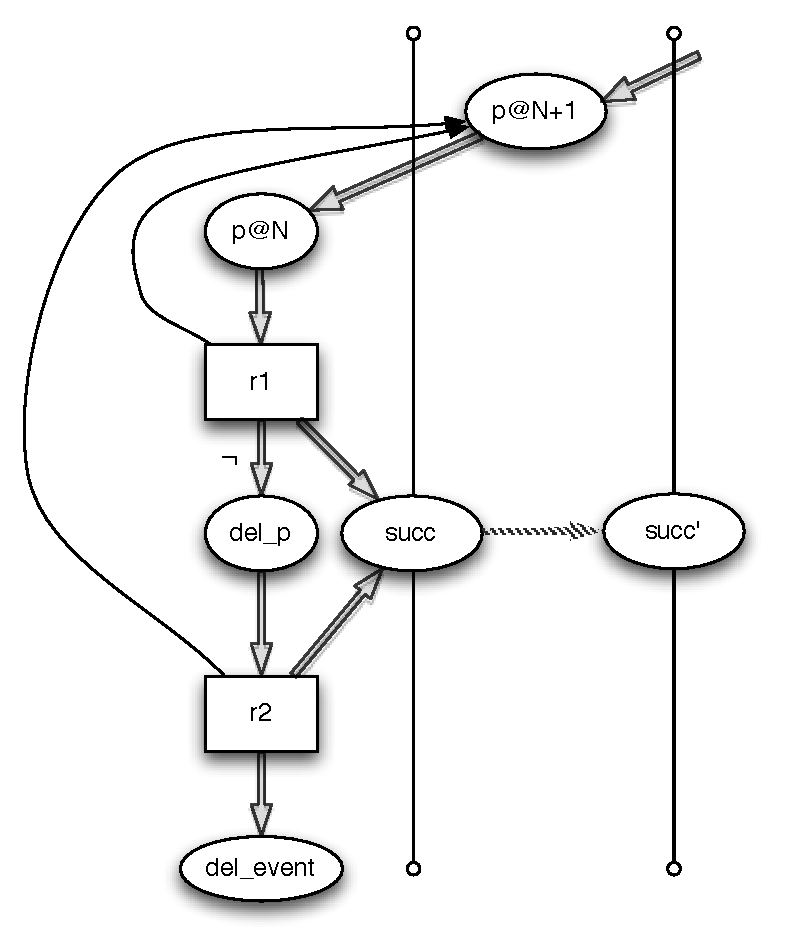
\includegraphics[width=0.75\linewidth]{localstrat_rgg.pdf}
  \label{fig:lstrat}
  \caption{Mutable persistence is locally stratified on time}
\vspace{-8pt}
\end{figure}


The difficulty with the continuous interpretation is that we must consider the \emph{successor} relation as infinite, which clearly leads
to unsafe programs.  To make matters worse, many useful programs that mutate state will be unstratifiable, because \emph{del\_p} predicate
will be defined negatively in terms of the positive \emph{p} predicate.  For example, take the program below in which \emph{insert\_p}
and \emph{delete\_p} are external events:

\begin{Dedalus}
r1
p(A, B, T)@N+1 \(\leftarrow\)
  p(A, B, T)@N,
  \(\lnot\)del\_p(A, B, T)@N;
  
r2
p(A, B, T)@N \(\leftarrow\)
  insert\_p(A, B, T)@N;

r3  
del_p(A, B, T)@N \(\leftarrow\)
  p(A, B, T)@N,
  delete\_p(T)@N;
\end{Dedalus}

This reasonable program is unstratifiable because $p \succ del\_p \land del\_p \succ p$.  But because the successor relation is constrained
such that $\forall A,B (successor(A, B) \rightarrow B > A)$, any such program is locally stratified on \emph{successor} (see \ref{fig:lstrat}).  Informally,
we have $p_{n+1} \succ del\_p_{n} \succ p_{n}$.

%%We sidestep these difficulties in two ways:

%%\begin{enumerate}
%%\item By joining \emph{now}, we only consider one finite partition (really, one value) of \emph{successor} in a given fixpoint.
%%\item Any finite partition of \emph{successor}, including any that we may consider in the post-hoc interpretation, is locally stratified. 
%%\end{enumerate}

\section{Cost Model}

%%\newdef{definition}{Definition}
Lemma~\ref{lem:cost} expresses that we can trade computation cost for storage 
cost in evaluation of a Dedalus program. 

%In the continuous interpretation of a Dedalus program, it is in general only
%useful to remember facts at a single timestamp in a predicate.  Two ways to
%approach this issue are to either always persist the ``latest'' version, or
%continuously re-derive the latest version.  These are represented in the naive
%deductive and overwriteable storage implementations below.

%\begin{figure}[t]
%\begin{tabular}{ll} \hline
%%Rule Pattern & Idiom & Prepare & Propose & Election \\ \hline \hline
%$d$ & Cost of a deductive step \\
%$s$ & Cost of storing a tuple \\
%$r$ & Cost of reading a tuple \\ 
%$t$ & Number of tuple derivations from deductive rules \\ 
%\hline
%$S$ & Set of tuples inserted \\
%$U$ & Set of tuples updated \\
%$P$ & Set of stored tuples, with time projected out \\ 
%$T$ & Set of stored tuple timestamps \\ 
%$Q$ & Set of query timestamps \\ \hline 
%\end{tabular}
%\caption{Cost model.}
%\label{fig:breakdown}
%\end{figure}


\subsubsection{Naive Deductive Implementation}

To evaluate a trace consisting of $S$ inserts and $U$ updates, a naive
deductive implementation would:

\begin{enumerate}

\item Add all inserts, deletions, and updates to the EDB.  
%We make the simplifying assumption that all EDB predicates are indexed by some
%hash of their key attributes.
Note that an update consists of both an insertion and a deletion.  Assuming
that inserting a fact into the EDB has some cost $w$ independent of the
characteristics of the predicate (e.g. all predicates store their facts in hash
tables), then the cost of this step is $(S+2U)w$.

\item For every predicate $P$, at time $M$, we must evaluate all predicates in
$P$'s predicate dependency graph at time $1$ through $M$.  
%A bottom-up evaluation of a predicate $P$ consists of evaluating all rules
%that reference $P$ in the head, and may involve polynomially many derivations
%in the size of the EDB up to time $M$.
A naive query plan for execution of a rule would consist of taking the cross
product of all body relations, selecting the subset that matches the body
conditions, and projecting this subset onto the head predicate to derive new
head tuples.  Assume each rule has an associated
selectivity $s_r$ and cost per each tuple in the join result $d_r$.  If a rule
is part of a recursion, it will be executed for $n_r$ steps.  The cost
of this evaluation is $M \cdot \sum_{r} n_r \cdot s_r \cdot d_r$.

\end{enumerate}

In summary, the total execution cost is:

\[ (S+2U)w + M \cdot \sum_{r : P \in r.head} n_r \cdot s_r \cdot d_r  \]

Since we only need persist the EDB, the total storage cost is equal to the size
of the EDB.

%$(|S|+2|U|)s + (|S|+2|U|)r + t + (\displaystyle\sum_{i=0}^{|Q|-1} \displaystyle\sum_{j=0}^{|T|-1} Q_{i} - T_{j})d$

\subsubsection{Naive Overwriteable Storage Implementation}

An overwritable storage implementation may enable lower execution latency by
storing the most recent version of a tuple.  For a predicate $P$ at time $M$,
we would need to evaluate each predicate $Q$ in $P$'s predicate dependency
graph from timestamp $Q_N+1$ through timestamp $M$ -- where $Q_N$ is the
timestamp of the last stored tuple of predicate $Q$. This is in contrast to the
naive deductive model, which would require computation from timestamp 1, but
would not require persisting the IDB of the most recently computed stratum for
each predicate.

In summary, the total execution cost is:

\[ (S+2U)w + \sum_{r} (M - Q_{r.head}) n_r \cdot s_r \cdot d_r  \]

The total storage cost is the IDB of each predicate at its most recent
timestamp.

%%\subsubsection{perhaps we can admit queries over the past that are bounded and pre-stated, and do GC}

\section{Implications for Distributed Systems}

\subsection{Space is simply time}

Dedalus programs can model many classes of distributed systems.  Consider the (distributed) dedalus program

\begin{Dedalus}
ping(@A, B)@(A, B, N) \(\leftarrow\)
  init(A, @B)@N; 

pong(@B, A)@r(A, B, N) \(\leftarrow\)
  ping(@A, B)@N;
\end{Dedalus}

And its rewrite in Datalog$\lnot$ with choice:

\begin{Dedalus}
ping(A, B, S) \(\leftarrow\)
  init(A, B, N),
  successor(N, S),
  choose((_), (S));

pong(B, A, S) \(\leftarrow\)
  ping(A, B, N),
  successor(N, S),
  choose((_), (S));
  
\end{Dedalus}

We may regard  \emph{r()} as a function over the attributes occurring in the body of the rule.  \wrm{I still think that time and the head predicate need to be inputs to r(), to ensure that duplicate facts are derived at the same time, and there are no implicit timing dependencies between facts in different predicates with the same key values.} The implementation or \emph{r()} is provided by
the model.  For example:

\subsubsection{Synchronous Systems}

r(\_) = 1 for all \_.  Computation proceeds in rounds.

\subsubsection{Asynchronous Systems}

The return value of r may be any arbitrary integer, positive or negative, including a NULL integer indicating an infinite value.

\subsubsection{Lamport Clocks}

As a middle ground, we might wish to enforce a constraint that $r(\_) > 0$.  Doing so would entail implementing a \emph{Lamport Clock}. 

\paa{part of me is considering dispensing with this r() stuff.  call it ``later", and define it in terms of choice over successor.  then the above enumeration
of ``implementations of $r$" becomes an enumeration of selection conditions to add to each ``later" rule}

\subsubsection{Synchronous Systems2}

We enforce that $S = N + 1$.

\subsubsection{Asynchronous Systems2}

%%The return value of r may be any arbitrary integer, positive or negative, including a NULL integer indicating an infinite value.
No selection; any row of successor, including the NULL row, is possible.

\subsubsection{Lamport Clocks2}

As a middle ground, we might wish to enforce a constraint that $S > N$.  Doing so would entail implementing a \emph{Lamport Clock}. 


\begin{figure}[t]
  \centering
  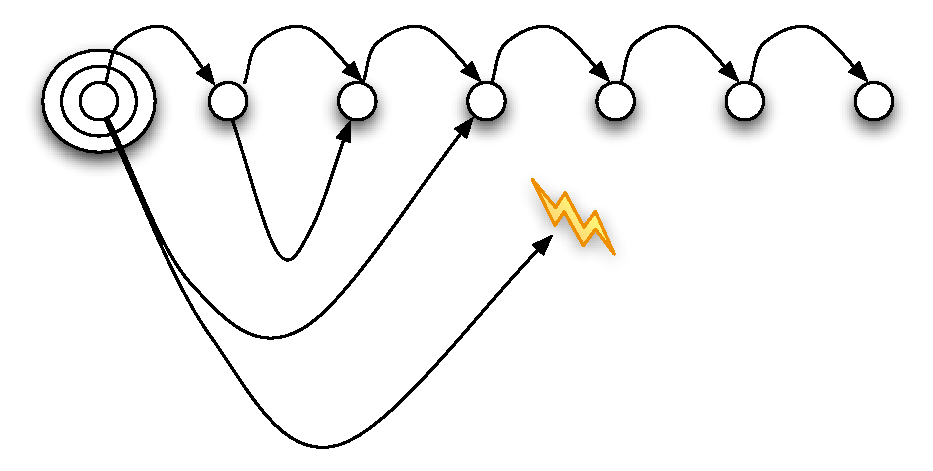
\includegraphics[width=0.75\linewidth]{dedalus-time.pdf}
  \label{fig:dedalus-time}
  \caption{Time moves forward in three ways: across strata, to the next fixpoint, and to some future fixpoint.}
\vspace{-8pt}
\end{figure}




\section{Correctness Criteria}

We introduce two correctness criteria for distributed systems: eventual consistency and confluence.

\subsection{Confluence}

{\em Confluence} means that there is a unique ultimate model.

When does a \lang program have a unique ultimate model?  While it is the presence of choice or asynchrony that causes multiple stable models, these multiple stable models sometimes give rise to a unique ultimate model.

\subsection{Eventual Consistency}

{\em Eventual consistency} means that all replicas eventually have the same replicated state, for any non-deterministic choices of time.  In other words, every ultimate model has the symmetry property that the contents of any replicated predicate is equivalent at all the replicas.  This is equivalent to the definition in (cite Peter's paper about EC).  Vogels' presented several operational definitions of eventual consistency \wrm{which are basically totally different, do we include here or not?  to discuss tomorrow}

\subsection{Space-Time Duality}

\wrm{discuss this more tomorrow}

%Eventual consistency and confluence are duals.
%Every eventually consistent program P has a confluent dual P', and every confluent program P' has an eventually consistent dual P.  Roughly, the transform is as follows.  We take our program, and have it only performs one node of the replication (nondeterministically commits to a node via committed choice???), and convert nondeterministic choice into replication (only a finite number of meaningful interleavings of messages -- how do we discover???), then this program is confluent iff the original program is E.C.


\begin{lemma}
Confluence of a \lang program is undecidable.
\end{lemma}
\begin{proof}
Our proof proceeds via construction of a two counter machine in \lang, inspired by the construction in \wrm{cite Levy} used to show that query satisfiability for Datalog with recursion and stratified negation is undecidable.  The construction is as follows:

The following relations are part of the program:
\dedalus{cnfg(S,C1,C2)}: Configurations of the machine, where \dedalus{S} is the state, and \dedalus{C1} and \dedalus{C2} are the values of the two counters.
\dedalus{fin\_succ(X,Y)}; A finite prefix of the successor relation, which is used for addition and subtraction of the counter values.

\wrm{fill in more code here}

The two counter machine performs committed choice after each transition to decide whether to halt in its current state or keep going.  The idea is that confluence is a property over all inputs to the two counter machine, and all choices of time.  So if, for some prefix of the infinite successor order, the two counter machine's early halting makes a difference in acceptance/rejectance only if the TM does not accept the empty language.  Therefore, if we can declare this program confluent, we have decided whether a 2cm accepts the empty language (which is a known undecidable problem). 

\end{proof}

%\begin{corollary}
%Eventual consistency of a \lang program is undeicdable.
%\end{corollary}
%\wrm{We need a bit more work in defining the spacetime duality to see if that's fully general.  If so, then there's a bijection between \lang programs defined by this duality, and the corollary will hold I think.}

The undecidability of the fully general cases leads us to consider subsets of the language, and conservative checks on the fully general class of programs (ala stratification).

\subsection{More Conservative Conditions}

Since \lang forces locality in time, the only source of non-determinism is non-determinism in co-occurence of truth of predicates.  This intuition implies a very natural conservative and statically checkable condition: force everything to eventually co-occur, and prevent observation of states where things have not yet co-occured.  The first property is asured by persisting all async messages.  The second is assured by ensuring that the EDB is related {\em monotonically} with the ultimate model.

\begin{definition}
If a {\em monotonic property} is true at time \dedalus{T}, then it is true at any time \dedalus{S > T}.
\end{definition}

An example of a monotonic property would be a persistent fact, or the negation of a fact that is never true.  Intuitively, a monotonic property represents some knowledge that never becomes untrue as we learn more knowledge.

\begin{definition}
A \lang program is {\em monotonic} if for all facts in the ultimate model, the element of the trace corresponding to the first time the fact was true before being henceforth true was computed by only monotonic properties. \wrm{may need some slight tweaking}
\end{definition}

\begin{example}
Example of a logically monotonic Dedalus program:\\
\begin{Dedalus}
node(X)@next <- node(X);
resposne(X)@next <- response(X);
all_responded() <- !not_responded(_);
not_responded(X) <- node(X), !response(X);
all_responded()@next <- all_responded();
\end{Dedalus}
\end{example}

The above program is monotonic. There is only one possible nonempty ultimate model, which contains \dedalus{all\_responded()}, and this fact is implied by a predicate \dedalus{!not\_responded(\_)}, which is monotonic because it is {\em r-positive} \wrm{cite Immerman} (i.e. the negation depth is even).  Note that the program is also confluent, because for any EDB, there is a unique ultimate model: either every node has an associated response, leading to a model with \dedalus{all\_responded()}, or there exists some node without an associated response, leading to an empty ultimate model.

We will see that all logically monotonic programs are confluent.  However, there are some non-logically-monotonic programs that are also confluent.

\begin{lemma}
A monotonic property must be true in all traces of a program, given an EDB.
\end{lemma}
\begin{proof}
Proof sketch: assume a monotonic property is true in one trace and false in another trace.  This means the monotonic property can differentiate between the two traces.  But since all async facts are persisted, all messages eventually rendezvous.  Thus, the monotonic property must be able to observe the condition that some event has not yet occured (but will eventually occur).  Monotonic properties cannot observe this though, becuase the property will be eventually untrue (when the thing that has not yet occured eventually occurs), thus it is not monotonic.
\end{proof}

\begin{corollary}
Logical monotonicity is a sufficient condition for confluence.
\end{corollary}
\begin{proof}
Proof sketch: if the ultimate model is populated only by monotonic properties, which are true in all traces, then there is a unique ultimate model.
\end{proof}

We now show that logical monotonicity is not necessary for confluence:

\begin{example}
Example of a confluent Dedalus program that is not logically monotonic:\\
\begin{Dedalus}
//client
b(#s,I)@async :- b_edb(I);

//server
b(N,I)@next <- b(N,I), !dequeued(I);
b_lt(i,j) <- b(_,i), b(_,j), i < j;
dequeued(i)@next <- b(_,i), !b_lt(_,i);
odd()@next <- odd(), !dequeued(_);
odd()@next <- dequeued(), even();
even() <- !odd();
\end{Dedalus}
\end{example}

The ultimate model contains \dedalus{odd()} if there are an odd number of \dedalus{b\_edb(I)} facts, and \dedalus{even()} otherwise.  Thus it is confluent.  However, the program is not logically monotonic because neither \dedalus{dequeued()} nor \dedalus{!dequeued()} are monotonic, so \dedalus{even()} is not supported by only monotonic properties, thus the program is not logically monotonic.

\wrm{Example of a Dedalus program that is nonconfluent (and thus not logically monotonic)}

\wrm{Making that program both monotonic and confluent via the addition of coordination}

\wrm{Logical monotonicity is undecidable?  Maybe a reduction from query satisfiability or something?}


\section{Conclusion and Future Work}

\jmh{In here, please follow up on the intro -- discuss how we built some serious shit in Overlog, and we believe that \lang is just 
as expressive because its operational semantics (cite boom-tr) are essentially the same as the behavior of Algorithm 1.  Formalizing this
a bit difficult since it entails developing a proper definition of the operational semantics of our Overlog interpreter.  Rather than trouble ourselves
with that, we are in the process of ``porting'' our Overlog code to Dedalus. }
Datalog has inspired a variety of recent applied work, which touts the benefits of declarative specifications for practical implementations.  Unfortunately, Datalog's declarative semantics make no guarantees
regarding the order in which derivations will occur; or rather, they derive all derivations in one atomic fixpoint computation.  This makes it difficult to associate natural ``side-effects'' like state update and message delivery with purely logical notions of deduction.


\lang is the result of our experience using hybrid
declarative/imperative languages such as Overlog~\cite{Loo2009-CACM}
to implement a number of networking protocols and distributed
systems~\cite{boom-techr,Alvaro2009I-Do-Declare:-C,Chu:2007,Loo2009-CACM}.
Although our experience with those languages was largely positive, the
combination of Datalog and imperative constructs hampered our
development of program analyses, and even our understanding of the
``correct'' execution of single-node programs that performed state
updates.

By mapping time to another type of data over which logical deductions
are performed, \lang allows us to express concepts such as asynchrony and state update in terms of a purely deductive logic
language, achieving the goal of a declarative language without sacrificing critically expressive features for the distributed systems domain.

\jmh{I think this paragraph says ``\lang handles state'', and the next says ``\lang handles asynchrony.''  Yes?  Let's say so than.}
At their core, state update and communication differ from logical
deductions only in terms of timing; \lang's notion of time allows us
to interleave operations and time in terms of logical deductions.
In the local case, this allows us to express state update without giving up the clean semantics of Datalog; unlike
Datalog extensions that use imperative constructs to provide such
functionality, each \lang rule expresses a logical invariant that will
hold over all program executions.  
\jmh{next sentence is lost of me.}
Our treatment of time in terms of
logical constraints allows us to model issues such as causality (and
``clever'' systems that observe causality violations) in a flexible
manner.

However, interactions with external processes, and primitives such as
asynchronous and unreliable communication introduce nondeterminism
which \lang models with \dedalus{choose}.  

Our hope is that modeling external process and events with a single
primitive will greatly simplify program analysis techniques.  Rather
than spending time and effort translating imperative code into sets of logical
invariants over program executions, analyses of \lang programs can
work directly against the invariants encoded by the program, allowing
them to focus on invocations of \dedalus{choose}, each of which
encodes some less easily avoided source of non-determinism and
ambiguity, such as a hardware failure or end-user.

\rcs{not really happy with the last paragraph; we should at least say some high-level thing about raising level of abstraction of programming, enabling more applications, etc, etc...}


\bibliographystyle{abbrv}
\bibliography{pods}

\appendix
\section{Proof of Lemma 1}
\begin{proof}
%First, we prove an isomorphism between stable models, and finite prefixes of stable models.  Scan a stable model of a program timestamp by timestamp.  
We first present an algorithm for computing ultimate models, and argue that the algorithm computes exactly the ultimate models of the \lang program.  We then argue this algorithm can be run on our operational formalism, and show how operational traces correspond with prefixes of stable models.

Any \lang program without asynchronous rules is a $\text{Datalog}_{1S}$ program, and the algorithm given in~\cite{tdd} computes its ultimate model in polynomial space\footnote{The class of {\em multi-seperable}~\cite{tdd-poly} \lang programs, which comprises all \lang programs $P$ with guarded asynchrony and persisted EDB, and their coordinations $\textsc{Coord}(P)$, can be executed in polynomial time in the size of the input.} in the size of the input.  The algorithm evalutes the program for $2^G + e$ consecutive timesteps, where $G$ is the number of instantiations of the non-temporal attributes of the program rules using all combinations of constants in the Herbrand Universe, and $e$ is the maximum timestamp of any EDB fact.  At each step, the algorithm updates information on observed periodicities of facts.  When the algorithm terminates, any fact with a periodicity of 1 is regarded as part of the ultimate model.

For asynchronous rules, the natural distributed analog of the above algorithm simultaneously executes one instance for each node \dedalus{n}, using values of $G$ and $e$ computed from $E_{\text{\dedalus{{\scriptsize n}}}}$.  Each instance has its own local clock, which corresponds to the timestamp attribute in the model-theoretic semantics.  Nodes communicate over channels with arbitrary delay and message re-ordering.  When a remote node \dedalus{m} derives a fact at \dedalus{n}, it encloses its local clock value, \dedalus{t}; \dedalus{n} must consider this fact at his local time \dedalus{t} or later, in the style of Lamport Clocks.  Note that this behavior is equivalent to the model-theoretic semantics of remote asynchronous rules: remote deductions are visible at the destination at a time later than the body temporal attribute at the source.  Further, note that Lamport Clocks only introduce the constraint that if message $a$ ``happens before'' $b$, in other words $a$ directly or transitively causes $b$ to be sent, then $T(a) < T(b)$.  If $a$ and $b$ are concurrent, there is some execution where $T(a) \geq T(b)$.

When \dedalus{n} processes a received message, the number of constants available to \dedalus{n} may increase, and thus the node's $G$ may increase to $G'$.  Furthermore, the node may need to execute over this new fact for $2^{G'}$ additional timesteps.  If only finitely many messages are sent, this algorithm terminates, and requires polynomial space.  In the case that infinitely many messages are sent, we only need to process each message $2^{G'}$ times: the maximum period of any fact is $2^{G'}$, as every incoming fact needs to have a chance (in some execution) to join with any deduction (with which it is ``concurrent'') at any time during its period.  Keeping track of the number of times we have seen each fact also requires polynomial space.  When the algorithm is done running for $2^{G'}$ steps, it pauses, waiting for new network input that it has not seen enough times.  If all nodes are paused and no outstanding messages exist, then the collection of all period 1 facts at all instances of the algorithm comprises an ultimate model.

We claim that the algorithm can generate every ultimate model---every message has the opportunity to join with another concurrent message or its transitive consequents at any point during their period, and has the opportunity to join with a causally related message during the range of times allowed by the model-theoretic constraint (identical to the Lamport Clock condition used in the algorithm).  Furthermore, the set of all facts, and their local timestamps, comprises a prefix of a stable model.

Note that we can execute this algorithm straightforwardly on our operational formalism.  Evaluating a single timestamp of a \lang program corresponds to the evaluation of a Datalog program, which is a polynomial time computation, and the Turing Machines can also maintain the necessary state about periods and message counts.
%2) Intuitively, the operational model is based on n Turing Machines, one per value of node(), which independently step sequentially through time and communicate via channels with
%non-deterministic delay.  At each timestep t they run a datalog fixpoint computation that evaluates P on ``projection(E_n, t)'' (notation needed); this takes polynomial
%time~\cite{immerman}.  At the end of this fixpoint there are three sets of relevant facts: local, synchronous facts that have timestep t+1 and become part of ``projection(E_n,
%t)'', local asynchronous facts whose timestep is chosen non-deterministically to be greater than t and become part of later timesteps, and remote asynchronous facts.  The
%timestamps in this third class of facts are chosen non-deterministically ``at the receiver'' to model delay, in a way that observes traditional causality
%restrictions~\cite{lamportclocks}.
%3) Any \lang program without  async rules is a Datalog_{1S} program, and the above intuition is captured by the algorithm given in~\cite{}, computing an ultimate model in
%polynomial space in the size of the input.  In the presence of asynchronous rules, this formalize needs to be expanded to account for the asynchronous advancement of time through
%\dedalus{successor} at each node.  The PSPACE guarantees of~\cite{} are not shown to hold for such programs, but in Appendix Foo we show that the following Lemma holds for all
%\lang programs under this model
\end{proof}

\section{Proof of Lemma 2}
\begin{proof}
We begin by assuming that \dedalus{node} contains the identifiers of each of the $n$ nodes.  Since the atemporal fragment of \lang is FO[LFP], we can represent a polynomial-time bounded Turing Machine using only atemporal rules in \lang~\cite{immerman-ptime}.  In addition to normal operations, the Turing Machine can place items into a queue---\cite{dedalus} shows how to model queues in \lang---or send messages to other nodes---modeled by an asynchronous communication rule with \dedalus{queue} in the head.  A node persists the contents of the tape across time if the queue is empty, using a rule like \dedalus{tape(\dbar{X})@next <- tape(\dbar{X}), !queue(\dbar{\_});}.  If the queue is non-empty, the computation skips a timestamp (leaving \dedalus{tape} empty), and then atomically copies the contents of \dedalus{queue} to \dedalus{tape}.  The ultimate model of this program is exactly the final contents of the tape on every node if the computation halts.  Otherwise, the program's ultimate model is empty: \dedalus{tape} facts only exist every other timestamp, and for any Turing Machine predicate \dedalus{r} we can create \dedalus{r'}, and create a mutual recursive cycle to ensure neither \dedalus{r} nor \dedalus{r'} contains facts at every timestamp:

\begin{Dedalus}
r(\dbar{X})@next <- r'(\dbar{X});
r'(\dbar{X})@next <- r(\dbar{X});
\end{Dedalus}

We can play a somewhat similar trick for \dedalus{queue} by having local messages alternate between going into \dedalus{queue} and \dedalus{queue'}.  Thus, no local queue message will be part of the ultimate model.  Remote messages will still go into \dedalus{queue}: this still leaves the case that the exact same message repeatedly arrives at a node at every timestamp forever, by chance.  We can dispense of this case by assuming the channels interconnecting the Turing Machines forbid it.
\end{proof}

\section{Proof of Lemma 3}
\begin{proof}
Our proof proceeds via construction of a two counter machine in \lang, inspired by the construction in~\cite{undecidable-datalog}.

We represent the state of a two counter machine using the \linebreak \dedalus{cnfg(T,S,C1,C2)} relation, where \dedalus{T} represents ``time'' (note this is not the same as the \lang temporal attribute), \dedalus{S} is the state, and \dedalus{C1} and \dedalus{C2} are the values of the two counters.  In order to support our two instructions, $inc$ and $dec$, we would like to make use of the \dedalus{successor} relation.  However, \lang conventions forbid the use of this infinite relation outside of the timestamp attribute.  Thus, we posit the \dedalus{fin\_succ(X,Y)} EDB relation, which is meant to represent a finite prefix of the \dedalus{successor} relation.  Since it is EDB, its contents may be arbitrary.  If \dedalus{fin\_succ} is malformed, then the machine's execution may be incorrect.  In particular, our model of the machine may accept an input, whereas the actual machine would not have accepted that input.  We illustrate how to constrain the contents of \dedalus{fin\_succ} below:

\begin{Dedalus}
malformed() <- fin_succ(_,0);
malformed() <- fin_succ(X,Y), fin_succ(X,Z), Y != Z;
malformed() <- fin_succ(Y,X), fin_succ(Z,X), Y != Z;
malformed() <- fin_succ(X,Y), X >= Y;
\end{Dedalus}

For a given EDB, the two counter machine either halts in the accepting state or halts in a non-accepting state.  It cannot run forever since the EDB (in particular, the \dedalus{fin\_succ} relation) is finite.

We construct a \lang program that nondeterministically decides to either run the machine on the input provided (and for the length of \dedalus{fin\_succ} provided, or declare that the machine will never accept without running it.  If the machine ever accepts some input, this induce two different ultimate models---one generated by a trace where we run the machine and it accepts, and one generated by a trace where we decide to not run the machine, and thus we implicitly reject.  We describe the program below. 

Initially, we nondeterministically decide whether to run the machine or not by sending two messages (0 and 1) to a remote node (\dedalus{decider}).  If both message arrive simultaneously, then the decider responds to run the machine.  Otherwise, the decider responds to declare failure:

%\jmh{should we use a hashmark for constants?  I would say no.}
\begin{Dedalus}
//send two messages to the decider
message(#D, 0)@async <- decider(D);
message(#D, 1)@async <- decider(D);

//decider responds to computer
run_machine(#computer)@async <- message(0),
                                message(1);
declare_failure(#computer)@async <- message(0),
                                    !message(1);
declare_failure(#computer)@async <- !message(0),
                                    message(1);
\end{Dedalus}

Each mapping in the transition function is expressed by a \lang rule with \dedalus{!malformed()} and \dedalus{!declare\_failure()} in its body.  For example, the rule $\delta(3, > =) = (7, inc, dec)$ would be represented as:

\begin{Dedalus}
cnfg(S,7,D1,D2) <- cnfg(T,3,C1,C2), C1 > 0, C2 == 0,
                   fin_suc(T, S), fin_succ(C1, D1),
                   fin_succ(D2, C2), !malformed(),
                   !declare_failure();
\end{Dedalus}

We declare success or failure as follows:

\begin{Dedalus}
reject() <- !accept();
accept() <- cnfg(20,_,_); //20 is the accepting state
accept()@next <- accept();
\end{Dedalus}

If we choose to declare failure, or the machine halts in a non-accepting state---whether it is due to incompleteness or malformedness of \dedalus{fin\_succ}, or actual halting---then the ultimate model will contain \dedalus{reject}.  If the machine halts in an accepting state, then the ultimate model will contain \dedalus{accept}.  Thus, if we can decide confluence of this program, then we can decide whether there is any input for which an arbitrary two-counter machine halts.
\end{proof}

\section{TRASH HEAP}

\paa{these are sections that I've cut}

\subsection{All sequence inputs are derived from time}

Input queues are simply a mapping between the ordering domain of the queue tuples and the time relation.  Naturally, this mapping
is infinite also and cannot be expressed as EDB.  But we can instead constructively state the rules that define how the mapping 
tracks the progress of the time relation.

Take a persistent relation q, associated with the following rule:

\begin{Dedalus}
q(A, B, O)@N+1 \(\leftarrow\)
  q(A, B, O)@N, 
  \(\lnot\)del\_q(A, B, O)@N;
\end{Dedalus}

In this example, the ordering domain $O$ is already given in the schema.  Like time, this queue may be viewed as an infinite stream.
To interact with a queue, we should be able to atomically dequeue an element in any timestep.  That is to say, in a given fixpoint computation,
we should be able to take an element from the queue such that in the next timestep that element is no longer there, regardless of the
underlying queue discipline.  Let's assume for a moment the existence of two helper predicates for operations on \emph{q}: \emph{sel\_q} and
\emph{deq\_q}.  


\begin{alltt}
begin_work(A, B, O)@N \(\leftarrow\)
  q(A, B, O)@N,
  event(A)@N, 
  sel_q(O)@N;
  
  
deq_q(O)@N \(\leftarrow\) 
  begin_work(_, _, O)@N;
\end{alltt}


To enforce an ordering on how we dequeue from the relation, we define a mapping between the ordering domain and the logical clock
time.  This mapping is likewise infinite and therefore may not be given as EDB.  However, we may express how to continually generate 
the mapping via a set of rules.

A trace may be interpreted as an entanglement of events and a local clock relation.

\subsubsection{Example 1: a FIFO queue}

\begin{Dedalus}
sel\_q(O)@N \(\leftarrow\)
  max\_q(O)@N;

max\_q(max<O>)@N \(\leftarrow\)
  q(\_, \_, O)@N;

del\_q(A, B, O)@N \(\leftarrow\)
  deq\_q(O)@N,
  q(A, B, O)@N;
\end{Dedalus}

\subsubsection{Example 2: per-host FIFOs}

\begin{Dedalus}
sel\_q(O)@N \(\leftarrow\)
  max\_q(_, O)@N; 

max\_q(A, max<O>)@N \(\leftarrow\)
  q(A, \_, O)@N;
\end{Dedalus}


\subsection{Dedalus Programs can be efficiently implemented}

:)

\subsubsection{Local stratification on time}

\subsubsection{Time is infinite but punctuated}

and indeed, so are any input streams.  we may dequeue as many events as we like from a given stream by using the mapping
between the elements in the queue and the time relation.  in the simplest case this mapping would be from the ordering domain 
of the queue to the time domain, but we can establish more complicated data-dependent mappings by including other attributes 
(e.g. we could implement QoS by including the address in the mapping and dequeueing a different number of items per host
per time unit).


%%\section{Proof of Lemma 1}
\begin{proof}
%First, we prove an isomorphism between stable models, and finite prefixes of stable models.  Scan a stable model of a program timestamp by timestamp.  
We first present an algorithm for computing ultimate models, and argue that the algorithm computes exactly the ultimate models of the \lang program.  We then argue this algorithm can be run on our operational formalism, and show how operational traces correspond with prefixes of stable models.

Any \lang program without asynchronous rules is a $\text{Datalog}_{1S}$ program, and the algorithm given in~\cite{tdd} computes its ultimate model in polynomial space\footnote{The class of {\em multi-seperable}~\cite{tdd-poly} \lang programs, which comprises all \lang programs $P$ with guarded asynchrony and persisted EDB, and their coordinations $\textsc{Coord}(P)$, can be executed in polynomial time in the size of the input.} in the size of the input.  The algorithm evalutes the program for $2^G + e$ consecutive timesteps, where $G$ is the number of instantiations of the non-temporal attributes of the program rules using all combinations of constants in the Herbrand Universe, and $e$ is the maximum timestamp of any EDB fact.  At each step, the algorithm updates information on observed periodicities of facts.  When the algorithm terminates, any fact with a periodicity of 1 is regarded as part of the ultimate model.

For asynchronous rules, the natural distributed analog of the above algorithm simultaneously executes one instance for each node \dedalus{n}, using values of $G$ and $e$ computed from $E_{\text{\dedalus{{\scriptsize n}}}}$.  Each instance has its own local clock, which corresponds to the timestamp attribute in the model-theoretic semantics.  Nodes communicate over channels with arbitrary delay and message re-ordering.  When a remote node \dedalus{m} derives a fact at \dedalus{n}, it encloses its local clock value, \dedalus{t}; \dedalus{n} must consider this fact at his local time \dedalus{t} or later, in the style of Lamport Clocks.  Note that this behavior is equivalent to the model-theoretic semantics of remote asynchronous rules: remote deductions are visible at the destination at a time later than the body temporal attribute at the source.  Further, note that Lamport Clocks only introduce the constraint that if message $a$ ``happens before'' $b$, in other words $a$ directly or transitively causes $b$ to be sent, then $T(a) < T(b)$.  If $a$ and $b$ are concurrent, there is some execution where $T(a) \geq T(b)$.

When \dedalus{n} processes a received message, the number of constants available to \dedalus{n} may increase, and thus the node's $G$ may increase to $G'$.  Furthermore, the node may need to execute over this new fact for $2^{G'}$ additional timesteps.  If only finitely many messages are sent, this algorithm terminates, and requires polynomial space.  In the case that infinitely many messages are sent, we only need to process each message $2^{G'}$ times: the maximum period of any fact is $2^{G'}$, as every incoming fact needs to have a chance (in some execution) to join with any deduction (with which it is ``concurrent'') at any time during its period.  Keeping track of the number of times we have seen each fact also requires polynomial space.  When the algorithm is done running for $2^{G'}$ steps, it pauses, waiting for new network input that it has not seen enough times.  If all nodes are paused and no outstanding messages exist, then the collection of all period 1 facts at all instances of the algorithm comprises an ultimate model.

We claim that the algorithm can generate every ultimate model---every message has the opportunity to join with another concurrent message or its transitive consequents at any point during their period, and has the opportunity to join with a causally related message during the range of times allowed by the model-theoretic constraint (identical to the Lamport Clock condition used in the algorithm).  Furthermore, the set of all facts, and their local timestamps, comprises a prefix of a stable model.

Note that we can execute this algorithm straightforwardly on our operational formalism.  Evaluating a single timestamp of a \lang program corresponds to the evaluation of a Datalog program, which is a polynomial time computation, and the Turing Machines can also maintain the necessary state about periods and message counts.
%2) Intuitively, the operational model is based on n Turing Machines, one per value of node(), which independently step sequentially through time and communicate via channels with
%non-deterministic delay.  At each timestep t they run a datalog fixpoint computation that evaluates P on ``projection(E_n, t)'' (notation needed); this takes polynomial
%time~\cite{immerman}.  At the end of this fixpoint there are three sets of relevant facts: local, synchronous facts that have timestep t+1 and become part of ``projection(E_n,
%t)'', local asynchronous facts whose timestep is chosen non-deterministically to be greater than t and become part of later timesteps, and remote asynchronous facts.  The
%timestamps in this third class of facts are chosen non-deterministically ``at the receiver'' to model delay, in a way that observes traditional causality
%restrictions~\cite{lamportclocks}.
%3) Any \lang program without  async rules is a Datalog_{1S} program, and the above intuition is captured by the algorithm given in~\cite{}, computing an ultimate model in
%polynomial space in the size of the input.  In the presence of asynchronous rules, this formalize needs to be expanded to account for the asynchronous advancement of time through
%\dedalus{successor} at each node.  The PSPACE guarantees of~\cite{} are not shown to hold for such programs, but in Appendix Foo we show that the following Lemma holds for all
%\lang programs under this model
\end{proof}

\section{Proof of Lemma 2}
\begin{proof}
We begin by assuming that \dedalus{node} contains the identifiers of each of the $n$ nodes.  Since the atemporal fragment of \lang is FO[LFP], we can represent a polynomial-time bounded Turing Machine using only atemporal rules in \lang~\cite{immerman-ptime}.  In addition to normal operations, the Turing Machine can place items into a queue---\cite{dedalus} shows how to model queues in \lang---or send messages to other nodes---modeled by an asynchronous communication rule with \dedalus{queue} in the head.  A node persists the contents of the tape across time if the queue is empty, using a rule like \dedalus{tape(\dbar{X})@next <- tape(\dbar{X}), !queue(\dbar{\_});}.  If the queue is non-empty, the computation skips a timestamp (leaving \dedalus{tape} empty), and then atomically copies the contents of \dedalus{queue} to \dedalus{tape}.  The ultimate model of this program is exactly the final contents of the tape on every node if the computation halts.  Otherwise, the program's ultimate model is empty: \dedalus{tape} facts only exist every other timestamp, and for any Turing Machine predicate \dedalus{r} we can create \dedalus{r'}, and create a mutual recursive cycle to ensure neither \dedalus{r} nor \dedalus{r'} contains facts at every timestamp:

\begin{Dedalus}
r(\dbar{X})@next <- r'(\dbar{X});
r'(\dbar{X})@next <- r(\dbar{X});
\end{Dedalus}

We can play a somewhat similar trick for \dedalus{queue} by having local messages alternate between going into \dedalus{queue} and \dedalus{queue'}.  Thus, no local queue message will be part of the ultimate model.  Remote messages will still go into \dedalus{queue}: this still leaves the case that the exact same message repeatedly arrives at a node at every timestamp forever, by chance.  We can dispense of this case by assuming the channels interconnecting the Turing Machines forbid it.
\end{proof}

\section{Proof of Lemma 3}
\begin{proof}
Our proof proceeds via construction of a two counter machine in \lang, inspired by the construction in~\cite{undecidable-datalog}.

We represent the state of a two counter machine using the \linebreak \dedalus{cnfg(T,S,C1,C2)} relation, where \dedalus{T} represents ``time'' (note this is not the same as the \lang temporal attribute), \dedalus{S} is the state, and \dedalus{C1} and \dedalus{C2} are the values of the two counters.  In order to support our two instructions, $inc$ and $dec$, we would like to make use of the \dedalus{successor} relation.  However, \lang conventions forbid the use of this infinite relation outside of the timestamp attribute.  Thus, we posit the \dedalus{fin\_succ(X,Y)} EDB relation, which is meant to represent a finite prefix of the \dedalus{successor} relation.  Since it is EDB, its contents may be arbitrary.  If \dedalus{fin\_succ} is malformed, then the machine's execution may be incorrect.  In particular, our model of the machine may accept an input, whereas the actual machine would not have accepted that input.  We illustrate how to constrain the contents of \dedalus{fin\_succ} below:

\begin{Dedalus}
malformed() <- fin_succ(_,0);
malformed() <- fin_succ(X,Y), fin_succ(X,Z), Y != Z;
malformed() <- fin_succ(Y,X), fin_succ(Z,X), Y != Z;
malformed() <- fin_succ(X,Y), X >= Y;
\end{Dedalus}

For a given EDB, the two counter machine either halts in the accepting state or halts in a non-accepting state.  It cannot run forever since the EDB (in particular, the \dedalus{fin\_succ} relation) is finite.

We construct a \lang program that nondeterministically decides to either run the machine on the input provided (and for the length of \dedalus{fin\_succ} provided, or declare that the machine will never accept without running it.  If the machine ever accepts some input, this induce two different ultimate models---one generated by a trace where we run the machine and it accepts, and one generated by a trace where we decide to not run the machine, and thus we implicitly reject.  We describe the program below. 

Initially, we nondeterministically decide whether to run the machine or not by sending two messages (0 and 1) to a remote node (\dedalus{decider}).  If both message arrive simultaneously, then the decider responds to run the machine.  Otherwise, the decider responds to declare failure:

%\jmh{should we use a hashmark for constants?  I would say no.}
\begin{Dedalus}
//send two messages to the decider
message(#D, 0)@async <- decider(D);
message(#D, 1)@async <- decider(D);

//decider responds to computer
run_machine(#computer)@async <- message(0),
                                message(1);
declare_failure(#computer)@async <- message(0),
                                    !message(1);
declare_failure(#computer)@async <- !message(0),
                                    message(1);
\end{Dedalus}

Each mapping in the transition function is expressed by a \lang rule with \dedalus{!malformed()} and \dedalus{!declare\_failure()} in its body.  For example, the rule $\delta(3, > =) = (7, inc, dec)$ would be represented as:

\begin{Dedalus}
cnfg(S,7,D1,D2) <- cnfg(T,3,C1,C2), C1 > 0, C2 == 0,
                   fin_suc(T, S), fin_succ(C1, D1),
                   fin_succ(D2, C2), !malformed(),
                   !declare_failure();
\end{Dedalus}

We declare success or failure as follows:

\begin{Dedalus}
reject() <- !accept();
accept() <- cnfg(20,_,_); //20 is the accepting state
accept()@next <- accept();
\end{Dedalus}

If we choose to declare failure, or the machine halts in a non-accepting state---whether it is due to incompleteness or malformedness of \dedalus{fin\_succ}, or actual halting---then the ultimate model will contain \dedalus{reject}.  If the machine halts in an accepting state, then the ultimate model will contain \dedalus{accept}.  Thus, if we can decide confluence of this program, then we can decide whether there is any input for which an arbitrary two-counter machine halts.
\end{proof}


\end{document}
